\documentclass[11pt,a4paper]{article}
\usepackage[margin=25mm]{geometry}
\usepackage[T1]{fontenc}
\usepackage{lmodern}
\usepackage{amsmath,amssymb,amsthm,mathtools}
\usepackage{graphicx,booktabs,array,microtype}
\usepackage[hidelinks]{hyperref}
\usepackage[nameinlink,noabbrev]{cleveref}
\newtheorem{theorem}{Theorem}
\newtheorem{proposition}[theorem]{Proposition}
\newtheorem{lemma}[theorem]{Lemma}
\newtheorem{corollary}[theorem]{Corollary}
\theoremstyle{remark}\newtheorem{remark}[theorem]{Remark}
\DeclareMathOperator{\TV}{TV}
\DeclareMathOperator{\per}{per}
\DeclareMathOperator{\diag}{diag}
\DeclareMathOperator{\off}{off}
\newcommand{\E}{\mathbb E}
\newcommand{\Prb}{\mathbb P}
\newcommand{\CF}{\mathrm{CF}}
\newcommand{\opt}{\mathrm{opt}}
\newcommand{\succp}{P_{\mathrm{succ}}}
\newcommand{\norm}[1]{\left\lVert#1\right\rVert}
% Generated by scripts/build_publication.py; all counts extracted from validated evidence.
\providecommand{\ErunCount}{756}
\providecommand{\SourceProbabilityCount}{1610}
\providecommand{\SourceBracketCount}{36}
\providecommand{\CalibrationCellCount}{45}

\title{Collision-Aware Certification and Resource Accounting\\for Photonic Graph Bisection}
\author{}
\date{24 November 2026}
\begin{document}
\maketitle
\begin{abstract}
A passive interferometer preserves photon number, but its outputs need not encode valid balanced graph partitions. We study when collision information permits a quantitative replacement of its full bosonic output law by independent distinguishable particles, and what this permits one to claim about photonic optimization. For orthonormal occupied orbitals, a positive floor $c$ on every nonzero output intensity and an expected collision-pair count $M<c^2/2$ imply an explicit total-variation bound with leading upper envelope $M/(2c)$ at fixed $c$. A balanced two-photon family makes this coefficient sharp at $c=1/2$; a growing balanced spectator family shows why collision probability alone is insufficient. We give a complete proof while identifying its established permanent, cycle and rounding ingredients. We also prove a finite source-selection phase diagram under uniform loss: Haar-averaged threshold feasibility has two candidate source sizes per attempt and four per injected photon. These are feasibility results, not graph-quality enrichment. Finally, a reconciliation of all \ErunCount{} archived equal-budget runs at $n=4,6,8$ finds lower mean final success for the bosonic model than for its independently trained distinguishable control at each size. The recorded data establish no optimization advantage. A locally tested, explicitly offline Perceval pilot specifies the measurements needed for a future hardware comparison; no QPU data are reported. Originality of the complete density composition remains an open attribution question.
\end{abstract}
\section{Introduction}

Balanced graph partitioning is a fundamental combinatorial optimization problem with applications in:
\begin{itemize}
    \item Load balancing in distributed computing
    \item Image segmentation
    \item Quantum circuit design
    \item HPC communication patterns
\end{itemize}

The Minimum Bisection problem seeks a partition of vertices into two equal-sized sets that minimizes the cut weight. Classical approaches use penalty-based QUBO formulations, but these introduce dense couplings and allow exploration of infeasible states.

Recent work in photonic quantum optimization has explored constraint-preserving approaches using photon-number conservation. In a passive linear interferometer, the total photon number is conserved, which could potentially replace penalty terms in the optimization.

This paper investigates whether photon-number conservation can provide a more natural constraint enforcement compared to penalty-based QUBO formulations. We develop a fixed-k photon interferometer approach, validate it on small instances, and compare with classical baselines.

\section{Physical and optimization model}\label{sec:model}
Let $G=([n],E,w)$ be a simple undirected graph with even $n$, finite nonnegative edge weights and no self-loops. A balanced binary partition $x$ obeys $\sum_i x_i=n/2$ and has cost
\begin{equation}
 C_G(x)=\sum_{\{i,j\}\in E}w_{ij}|x_i-x_j|.\label{eq:cut}
\end{equation}
The strings $x$ and $1-x$ have the same cost but are distinct detection events. Exact enumeration uses both strings consistently when computing success probabilities. Symmetry reduction for classical search must not divide physical event counts by two.

For the direct encoding set $m=n$ modes and $k=n/2$ injected single photons in distinct inputs. More generally let $V\in\mathbb C^{m\times k}$ be the occupied columns of a passive lossless unitary, so $V^\dagger V=I_k$. The normalized bosonic input after the interferometer is $\prod_{a=1}^k(\sum_iV_{ia}a_i^\dagger)|0\rangle$. An output is a Fock occupation $t\in\mathbb N^m$ with $|t|=k$. Choose any list $y=(y_1,\ldots,y_k)$ with these multiplicities and write $t!=\prod_i t_i!$. The full laws for indistinguishable bosons and independent distinguishable particles with labels forgotten are
\begin{equation}
 p_b(t)=\frac{\left|\sum_{\sigma\in S_k}\prod_jV_{y_j,\sigma(j)}\right|^2}{t!},\qquad
 p_d(t)=\frac{\sum_{\sigma\in S_k}\prod_j|V_{y_j,\sigma(j)}|^2}{t!}.\label{eq:laws}
\end{equation}
Repeated output rows and their factorials are retained. The full Fock space has dimension $\binom{m+k-1}{k}$, whereas the collision-free sector has $\binom{m}{k}$ occupations. At $m=8,k=4$ these are $330$ and $70$. Photon-number conservation does not restrict the law to the latter sector; Hong--Ou--Mandel bunching gives the elementary counterexample~\cite{hom1987}.

Let $F=\{t:|t|=k,\ t_i\le1\}$ denote valid direct encodings, and let $O_G\subset F$ be the set with minimum cut cost $C^*$. For an ideal injected attempt,
\begin{equation}
 P_F=p(F)=P_{\CF},\quad P_{\opt\mid F}=p(O_G)/p(F),\quad
 \succp=p(O_G)=P_F P_{\opt\mid F}.\label{eq:success}
\end{equation}
The conditional probability is undefined if $P_F=0$. Under loss, having no collision does not imply having $k$ photons: vacuum and one-photon outcomes are also collision-free. Then $F$ must retain the condition $|t|=k$. In experiments, the denominator must specify emission attempts, successful injection, triggered acquisitions, or postselected detections. Without a measured attempt count, success per emission attempt is unidentified.

Conditional energy $\E[C_G\mid F]$ is a valid accessible training statistic, but its acceptance cost must be reported. The subnormalized moment $\sum_{t\in F}p(t)C_G(t)$ alone can reward rejecting costly states. Examples of optimum-blind losses are
\begin{equation}
 L_\mu=\E[C_G\mid F]+\mu(1-P_F),\qquad
 L_\gamma=\E[C_G\mid F]-\gamma\log P_F,\label{eq:train}
\end{equation}
and conditional lower-tail CVaR. An unconditional alternative assigns every rejected event an explicit cost $R\ge\max_{t\in F}C_G(t)$; $R=\sum_Ew_{ij}$ is available without solving the graph. With finite shots, normalization and no-valid-event handling require an explicit estimator. Our safe API accepts costs and feasibility but no $C^*$ or optimal-state mask. It does not make exact distribution access free.

By contrast, optimizing $p(O_G)$ requires knowledge of $C^*$. Such runs diagnose oracle-assisted state preparation. Once an optimal string is known, a permutation of occupied modes prepares it deterministically and gives $p(O_G)=1$. Identity gives $P_F=1$ and $P_{\opt\mid F}\in\{0,1\}$ according to whether its particular string is optimal, not a uniform average.

\section{A density-qualified certificate for independent particles}\label{sec:certificate}
Define $q_{ia}=|V_{ia}|^2$, row intensity $a_i=\sum_aq_{ia}$, dominant-support leakage $\delta$, and the bosonic collision-pair moment $M$ by
\begin{equation}
 \delta=\sum_i(a_i-\max_aq_{ia}),\qquad
 M=\sum_i\left(a_i^2-\sum_aq_{ia}^2\right)
   =\E_b\sum_i\binom{t_i}{2}.\label{eq:moment}
\end{equation}
The last identity follows by applying two annihilation operators to the occupied single-photon state: $\E_b[t_i(t_i-1)]=4\sum_{a<b}q_{ia}q_{ib}$. For distinguishable particles the pair moment is $M/2$. In general $M$ is not the probability of at least one collision. If $k\ge2$, then $1-P_{\CF}\le M\le\binom{k}{2}(1-P_{\CF})$ in the bosonic law.

For $0\le s<1$ and $x\ge0$ put
\begin{equation}
 f(s)=\frac12\left(\frac{e^{-s}}{1-s}-1\right),\quad
 \rho(x)=2\sqrt{x}+x,\quad
 \Phi(x)=\begin{cases}\min\{1,f(\rho(x))\},&\rho(x)<1,\\1,&\rho(x)\ge1.\end{cases}\label{eq:envelope}
\end{equation}
Throughout, $\TV(p,d)=\tfrac12\sum_t|p(t)-d(t)|$ on the complete unconditioned output space.

\begin{theorem}[Density and expected-collision certificate]\label{thm:density}
Let $V^\dagger V=I_k$, with one identical photon in each distinct occupied input. Suppose $c>0$ satisfies $a_i\ge c$ for every $a_i>0$. Then
\begin{equation}
 \delta\le M/c,\qquad \TV(p_b,p_d)\le\Phi(\delta)\le\Phi(M/c).\label{eq:coarse}
\end{equation}
If $M<c^2/2$, define
\begin{equation}
 d_c(M)=\frac{c-\sqrt{c^2-2M}}2
       =\frac{M}{c+\sqrt{c^2-2M}}.
\end{equation}
Then $\delta\le d_c(M)$ and $\TV(p_b,p_d)\le\Phi(d_c(M))$. At fixed $c>0$, the latter upper envelope is $M/(2c)+O(M^{3/2})$ as $M\to0$.
\end{theorem}
The floor applies to every positive row, including tiny ones. Average density $k/m$ is not a substitute. Exact zero rows may be removed. The asymptotic is an upper-envelope expansion, not an equivalence for every circuit or a uniform statement as $c\to0$.

\subsection{Proof of the certificate}
The spatial magnitude Gram matrix and its Frobenius deviation are
\begin{equation}
 B_{ab}=\sum_i\sqrt{q_{ia}q_{ib}},\qquad \sigma=\norm{B-I_k}_F.\label{eq:gram}
\end{equation}
This $B$ is not the internal-state distinguishability Gram matrix. In particular $B_{aa}=1$, and it generally has nonzero off-diagonal entries even for perfectly identical photons. We first record the permanent and cycle bounds; their complete elementary derivations are in \cref{app:gram}.
\begin{lemma}[Spatial overlap bounds]\label{lem:gram}
For the full laws in \cref{eq:laws},
\begin{equation}
 \TV(p_b,p_d)\le\min\{1,(\per B-1)/2\}.
\end{equation}
For real symmetric nonnegative $A=B-I_k$ and $\sigma=\norm A_F<1$,
\begin{equation}
 \per(I_k+A)-1\le e^{-\sigma}/(1-\sigma)-1.
\end{equation}
Without $\sigma<1$, the finite bound $\per(I_k+A)-1\le\sum_{r=2}^k(!r/r!)\sigma^r$ remains valid, where $!r$ counts derangements.
\end{lemma}

Assign each row to one maximizer $g(i)$ of $q_{ia}$, using any fixed tie rule, and let $S_g$ be the resulting partition. Define $C_{ga}=\sqrt{\sum_{i\in S_g}q_{ia}}$. Each column of $C$ has norm one. Write $C=D+E$ with $D$ diagonal and $E$ zero-diagonal. The discarded mass is $\norm E_F^2=\delta$, and $\norm D_{\mathrm{op}}\le1$. Groupwise Cauchy--Schwarz gives $B_{ab}\le(C^TC)_{ab}$ with equal diagonals. Consequently
\begin{align}
 \sigma&\le\norm{\off(C^TC)}_F\nonumber\\
 &\le\norm{DE}_F+\norm{E^TD}_F+\norm{\off(E^TE)}_F
 \le2\sqrt\delta+\delta.\label{eq:support}
\end{align}
The last step uses $\norm{E^TE}_F\le\norm E_F^2$. No dimension factor is introduced. Since $f$ is increasing on $[0,1)$, \cref{lem:gram} gives $\TV\le\Phi(\delta)$, with the trivial cap used when the majorant does not converge.

For each row put $h_i=\max_aq_{ia}$ and $d_i=a_i-h_i$. Then $\sum_aq_{ia}^2\le h_ia_i$, so $M\ge\sum_i a_id_i\ge c\delta$. For the refinement the off-maximum squared sum is at most $d_i^2$, whence
\begin{equation}
 M\ge\sum_i2d_i(a_i-d_i)\ge2c\delta-2\sum_i d_i^2
 \ge2c\delta-2\delta^2.\label{eq:quadratic}
\end{equation}
This quadratic alone does not select its small branch. The independent coarse bound and $M<c^2/2$ imply $\delta<c/2$, where $2\delta(c-\delta)$ is increasing. Inversion gives $\delta\le d_c(M)$. Finally $f(s)=s^2/4+O(s^3)$, $\Phi(x)=x+O(x^{3/2})$ near zero, and $d_c(M)=M/(2c)+O(M^2)$ at fixed $c$. This proves \cref{thm:density}.

\subsection{Sharpness and the need for a density hypothesis}
Let $m=4,k=2$, $w_1=(1,1,0,0)^T/\sqrt2$, $w_2=(0,0,1,1)^T/\sqrt2$, and take occupied columns $v_1=\cos\theta\,w_1+\sin\theta\,w_2$, $v_2=-\sin\theta\,w_1+\cos\theta\,w_2$, with $0\le\theta<\pi/4$. Direct enumeration of all ten Fock occupations gives
\begin{equation}
 a_i=1/2,\quad\delta=2\sin^2\theta,\quad
 M=\TV(p_b,p_d)=2\cos^2\theta\sin^2\theta
 =\delta(1-\delta/2).\label{eq:sharp}
\end{equation}
For example, the probabilities of photon totals $(2,0),(1,1),(0,2)$ in the two disjoint mode groups are $(2u,(1-2\epsilon)^2,2u)$ for bosons and $(u,(1-\epsilon)^2+\epsilon^2,u)$ for distinguishable particles, where $\epsilon=\sin^2\theta$ and $u=\epsilon(1-\epsilon)$. Within each grouped outcome the physical splitting laws agree. Their positive probability differences sum to $2u$, proving the full-law identity. Thus the leading coefficient $1/(2c)=1$ at $c=1/2$ cannot be reduced uniformly. This family has an elementary classical sampler.

Now take two flat occupied columns on even $L$ modes, one with all entries $1/\sqrt L$ and the other with half $+1/\sqrt L$ and half $-1/\sqrt L$. They are orthonormal. Their bosonic collision probability is $2/L$, but $\TV(p_b,p_d)=1/2$: same-sign distinct outputs have twice the distinguishable probability, and opposite-sign outputs are suppressed. For even $k$ choose $L=k+2$ and add $k-2$ deterministic spectator photons on isolated modes, yielding $m=2k$. Then
\begin{equation}
 1-P_{\CF}=M=2/(k+2)\longrightarrow0,\qquad
 \TV(p_b,p_d)=1/2.\label{eq:spectator}
\end{equation}
Here $c=2/(k+2)$ also tends to zero. Balanced average density alone therefore does not rescue a collision-only certificate. This is a counterexample to a particular independent-particle approximation, not evidence of classical hardness.

\subsection{Operational and numerical scope}
For any fixed event $E$, including optimal valid bisections, $|p_b(E)-p_d(E)|\le\TV(p_b,p_d)$. This compares the \emph{same} interferometer. It does not order separately optimized models or bound relative gains when both event probabilities vanish. An exact toy family with a twofold rare-event ratio and diverging waiting times is retained in the archive; a disclosed correlated classical control solves that toy case.

The quantities $a_i$ and $M$ are low-order number moments; inferring the minimum positive intensity with finite data is difficult without structural assumptions. Certifying the absence of tiny unobserved rows is an additional statistical problem. Current floating implementations are numerical diagnostics, not outward-rounded certificates: a retained tiny-angle cancellation witness refutes a literal exact-upper-bound interpretation of their returned floats. The exact theorem is independent of this numerical limitation.

\section{Uniform loss and the resource-dependent source optimum}\label{sec:loss}
For the direct $N=k$ encoding, uniform independent transmission $\eta$ retains all photons with probability $\eta^k$. If validity requires all $k$ photons, a fixed ideal success probability obeys
\begin{equation}
 \succp(\eta)=\eta^k\succp(1).\label{eq:all_detected}
\end{equation}
The illustrative inputs $k=4$, $\eta=0.9$, $\succp(1)=0.537$ give $0.3523257$, not $0.381$. This is an arithmetic model check, not an experimental datum or a reproduced optimized-circuit result.

A different source protocol accepts exactly $k=m/2$ \emph{threshold clicks}, allowing $N\ge k$ injected photons and output collisions or losses. It must not be conflated with direct $N=k$ collision-free encoding. For $\ell$ surviving photons and a Haar mode unitary, the known averaged acceptance law~\cite[Lemma 1, Eq.~(6), v2]{bouland2023} is
\begin{equation}
 h(\ell)=\frac{\binom{m}{k}\binom{\ell-1}{k-1}}{\binom{m+\ell-1}{\ell}}\quad(\ell\ge k),\qquad h(\ell)=0\quad(\ell<k).\label{eq:haar_click}
\end{equation}
For clarity, Haar averaging is uniform on Fock compositions; it is not a claim that a fixed interferometer has this law. With distinct single-photon inputs and uniform loss, survival sectors commute through the interferometer. Thus, for $L\sim\mathrm{Bin}(N,\eta)$,
\begin{equation}
 S_N(\eta)=\E h(L),\qquad b_N(\eta)=S_N(\eta)/N.\label{eq:source}
\end{equation}
All attempts, including vacuum, count in $S_N$.

\begin{theorem}[Two resource objectives, different source choices]\label{thm:source}
Let $m\ge8$ be even, $k=m/2$, $k\le N\le m$, and $0<\eta<1$.
\begin{enumerate}
\item The maximizer of $S_N$ lies in $\{m-1,m\}$. A unique $a_m\in(0,1)$ satisfies $S_m(a_m)=S_{m-1}(a_m)$. The optimum is $m$ below $a_m$ and $m-1$ above it.
\item The maximizer of $b_N$ lies in $\{m-3,m-2,m-1,m\}$. The adjacent crossings $b_{j+1}(\tau_j)=b_j(\tau_j)$ are unique and obey
\begin{equation}
 0<\tau_{m-1}<\tau_{m-2}<\tau_{m-3}<1.
\end{equation}
As $\eta$ decreases, the unique optimum is successively $m-3,m-2,m-1,m$. Only adjacent candidates tie at each crossing.
\end{enumerate}
At $\eta=1$, $S_N$ is maximized by both $m-2,m-1$ and $b_N$ uniquely by $m-3$.
\end{theorem}
\begin{proof}[Proof strategy]
The exact ratios are
\begin{equation}
 \frac{h(\ell+1)}{h(\ell)}=\frac{\ell(\ell+1)}{(\ell-k+1)(m+\ell)},\qquad
 \frac{g(\ell+1)}{g(\ell)}=\frac{\ell^2}{(\ell-k+1)(m+\ell)},\quad g(\ell)=h(\ell)/\ell.
\end{equation}
Their adjacent differences change sign once. Adding one independent Bernoulli survivor gives $S_{N+1}-S_N=\eta\E\Delta h(L)$, $L\sim\mathrm{Bin}(N,\eta)$. Size bias gives $b_{N+1}-b_N=\eta^2\E\Delta g(R+1)$, $R\sim\mathrm{Bin}(N-1,\eta)$. The one-crossing lemma in \cref{app:source} proves uniqueness and orders the crossings, excluding nonadjacent hidden maxima. That appendix supplies the complete argument.
\end{proof}

For fixed $\lambda\ge0$, $\eta=1-\lambda/m$ and fixed $s\ge1$, the boundary expansions are
\begin{equation}
 \frac{S_{m-s+1}}{S_{m-s}}-1=\frac{s+\lambda-2}{2m}+O(m^{-2}),\quad
 \frac{b_{m-s+1}}{b_{m-s}}-1=\frac{s+\lambda-4}{2m}+O(m^{-2}).\label{eq:boundary}
\end{equation}
Accordingly $m(1-a_m)\to1$, while the three per-photon crossing losses tend to $1,2,3$ in the corresponding order. These statements concern losses of order one photon; they are not fixed-transmission asymptotics. The proof and tail control are in \cref{app:source}. Exact rational finite checks verify \SourceProbabilityCount{} values and \SourceBracketCount{} root brackets; the checks do not prove the all-$m$ statement.

\begin{figure}[tb]
 \centering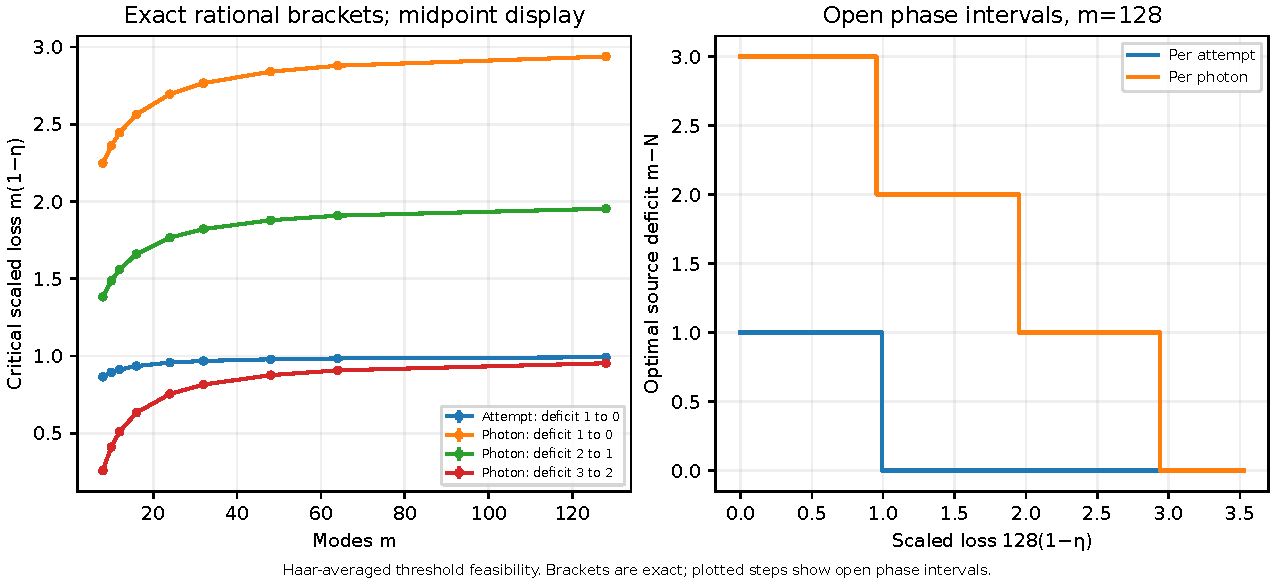
\includegraphics[width=\linewidth]{figures/fig_loss_source.pdf}
 \caption{Resource-dependent source transitions from the archived exact rational brackets. Lines display bracket midpoints; their widths are numerical root enclosures, not statistical uncertainty. The sequences approach the boundary limits proved in the text. The finite diagram counts all attempts and concerns Haar-averaged feasibility only.}\label{fig:loss}
\end{figure}
\begin{table}[t]
\centering
\begin{tabular}{ccc}
\hline
$\eta$ & Best $N$ per attempt & Best $N$ per injected photon \\
\hline
$\frac{3}{4}$ & $8$ & $7$ \\
$\frac{9}{10}$ & $7$ & $6$ \\
$\frac{99}{100}$ & $7$ & $5$ \\
$1$ & $6, 7$ & $5$ \\
\hline
\end{tabular}
\caption{Exact source choices from the preserved P37 rational grid at $m=8$, targeting exactly $m/2$ threshold clicks. All maximizing sources are listed, including ties. The criteria maximize success per attempt and success divided by injected photon number, respectively. This is Haar-averaged feasibility with loss, not graph optimization or a fixed-device waiting-time claim.}
\label{tab:losses}
\end{table}


Accepted Haar-averaged click subsets are uniform by mode symmetry, so improving $S_N$ does not preferentially produce good graph cuts. Moreover $N/S_N$ is a first-success photon cost only if Haar draws are independently refreshed between attempts. Drawing a Haar unitary once and fixing it instead involves $\E_U[N/p_U]$, which need not equal $N/\E_U p_U$ and can diverge. Neither expression includes programming, source preparation or classical optimization costs. Fixed total photon-budget allocation is a separate problem.

\section{Reconciled computations and negative optimization result}\label{sec:experiments}
\subsection{Evidence selection and elementary controls}
The repository retains both successful and failed campaigns. We reconstructed tables from recorded configurations, per-run outputs and training count traces, rather than from the previous manuscript. A source-hash inventory distinguishes byte-verified outputs, source-snapshot gaps, preserved failed attempts and unattributed copies. Historical driver scripts that overwrite fixed paths were not rerun. The new reconciliation is a deterministic analysis of the archive, not an independent repetition of every optimization trajectory.

An independent exhaustive check of all $64$ simple unweighted four-vertex graphs verifies costs, complementary partitions and exact minima. \Cref{tab:graphs} records representative graphs. Haar averaging gives a uniform law on the $D=\binom{m+k-1}{k}$ Fock compositions, so $\E P_{\CF}=\binom{m}{k}/D$ and $\E\succp=g^*/D$, where $g^*$ is the number of optimal valid \emph{strings}. At $m=4,k=2$, $D=10$. All six balanced strings are optimal on $K_4$, giving $\E\succp=0.6$; $K_{2,2}$ has minimum cut $2$ and four optimal strings, giving $0.4$. A graph-independent Haar success value $0.2$ is therefore incorrect. The Haar baseline is an ensemble average, not a universal per-circuit ceiling~\cite{arkhipov2012}.
\begin{table}[t]
\centering
\begin{tabular}{lrrc}
\hline
Graph & $C^*$ & Optimal strings $g$ & Haar $\mathbb{E}[P_{\rm opt}]$ \\
\hline
Path & 1 & 2 & $\frac{2}{10}$ \\
Cycle & 2 & 4 & $\frac{4}{10}$ \\
$K_4$ & 4 & 6 & $\frac{6}{10}$ \\
$K_{2,2}$ & 2 & 4 & $\frac{4}{10}$ \\
Star & 2 & 6 & $\frac{6}{10}$ \\
\hline
\end{tabular}
\caption{Computed four-vertex, two-photon controls. Balanced bitstrings and their complements are counted separately. The last column is a Haar ensemble expectation, not a trained or measured hardware success rate.}
\label{tab:graphs}
\end{table}


The E01 Haar archive includes size-dependent circuit counts; in particular the $n=10$ sample is smaller than the $n\le8$ samples. It does not provide trained $n=10,12$ optimization evidence. E02 uses the optimal-state mask during optimization and is retained as an oracle-assisted state-preparation diagnostic. E03--E04 compare small-instance objective/optimizer variants, while E06--E09 test structural baselines, spectral information, coherence diagnostics and label sensitivity. None warrants extrapolating a favorable oracle/Haar ratio to an optimum-blind algorithm.

\subsection{Exactly recorded query and attempt budgets}
The primary empirical comparison is E05b. The full grid has $n=4,6,8$, six graph families, two nominal graph seeds, three training seeds and seven method configurations: bosonic and distinguishable meshes, a classical iid multinomial control, a uniform feasible sampler, and classical product-Bernoulli penalty controls at three strengths ($0.1,1,10$). Repeated graph seeds can generate identical graphs; the nominal twelve graph positions at each size contain only $9,9,10$ unique edge lists, respectively. The archived global means retain the nominal grid weighting so the analysis does not select favorable graphs. Intervals use 2000 deterministic percentile bootstrap replicates with the $2.5$th and $97.5$th percentiles: a resampled graph cluster contributes all its optimizer repeats and nominal slots, and the replicate mean is the ratio of their summed probabilities to their record count. These intervals describe this fixed graph grid, rather than a random graph population; resampling seeds as independent graphs would inflate the evidence.

Each optimized trajectory records $120$ objective evaluations, $256$ ideal sampled attempts per evaluation, and a final $4096$-attempt batch: $120\times256+4096=34816$ attempts. This equality does not make classical matrix simulation costs equal to physical circuit shots or to a discrete-search query. Mesh dimension is obtained from its actual coupler list and phases, not equated to the number of Bernoulli parameters. Rejected/colliding outcomes remain in the denominator. For the bosonic, distinguishable and iid multinomial arms, training minimizes the sampled conditional cut plus $2(1-\widehat P_F)$. A batch with no valid outcome receives the fixed value $\sum_E w_{ij}+3$. Penalty arms minimize the sampled full binary QUBO energy. COBYLA uses a 120-call cap, initial radius $0.35$ and tolerance $10^{-7}$; any unspent calls follow a fixed Gaussian local-proposal completion rule of standard deviation $0.1$. Uniform feasible sampling has no trained parameters but spends the same draw budget.

At sizes $n=4,6,8$, the fitted mesh/iid arms train $n(n-1)=12,30,56$ real parameters, with the $n$ input phases fixed because they do not affect fixed-input Fock probabilities. Bernoulli arms train $n=4,6,8$ logits. These dimensions differ. The simulator retains the total non-CF mass as an explicit rejection category, without resolving its internal collision histogram; for $k\ge3$ these unresolved rejection counts do not generally determine the pair moment $M$. In the two-photon bosonic arm, however, every collisional outcome contains one pair and $M=1-P_{\CF}$ exactly. Table~\ref{tab:e05b} and \cref{fig:e05b} show the exact final distribution probabilities after finite-shot training, rather than the noisy success rates in the independent 4096-draw heldout batches. The retrospective optimum is used for evaluation, not the E05b recorded training loss; anti-oracle tests enforce that separation in the recovered public training API.

\begin{table}[t]
\centering\small
\setlength{\tabcolsep}{3pt}
\begin{tabular}{lccc}
\hline
Method & $n=4$ & $n=6$ & $n=8$ \\
\hline
Bosonic & \shortstack{0.652\\{[0.464, 0.804]}} & \shortstack{0.280\\{[0.178, 0.423]}} & \shortstack{0.068\\{[0.033, 0.107]}} \\
Distinguishable & \shortstack{0.713\\{[0.590, 0.835]}} & \shortstack{0.537\\{[0.389, 0.646]}} & \shortstack{0.138\\{[0.075, 0.197]}} \\
Classical iid multinomial & \shortstack{0.421\\{[0.310, 0.532]}} & \shortstack{0.110\\{[0.063, 0.158]}} & \shortstack{0.026\\{[0.016, 0.036]}} \\
Product Bernoulli penalty ($\lambda=0.1$) & \shortstack{0.199\\{[0.135, 0.268]}} & \shortstack{0.057\\{[0.033, 0.089]}} & \shortstack{0.017\\{[0.010, 0.023]}} \\
Product Bernoulli penalty ($\lambda=1$) & \shortstack{0.203\\{[0.141, 0.271]}} & \shortstack{0.056\\{[0.032, 0.088]}} & \shortstack{0.016\\{[0.010, 0.023]}} \\
Product Bernoulli penalty ($\lambda=10$) & \shortstack{0.199\\{[0.127, 0.270]}} & \shortstack{0.056\\{[0.032, 0.092]}} & \shortstack{0.017\\{[0.010, 0.023]}} \\
Uniform feasible & \shortstack{0.528\\{[0.333, 0.718]}} & \shortstack{0.175\\{[0.100, 0.277]}} & \shortstack{0.060\\{[0.036, 0.086]}} \\
\hline
\end{tabular}
\caption{Ideal final success means over 36 runs per method and size, with descriptive graph-cluster percentile intervals. There are 12 nominal graph slots per size but $G=9,9,10$ unique labeled weighted graphs, respectively. Every run uses 120 calls of 256 training draws plus 4096 heldout draws (34816 ideal attempts). Optimizer repeats stay in the same graph cluster; these are not population significance intervals. Each penalty parameter is a separate fully charged run. No hardware shots.}
\label{tab:e05b}
\end{table}

\begin{figure}[tb]
 \centering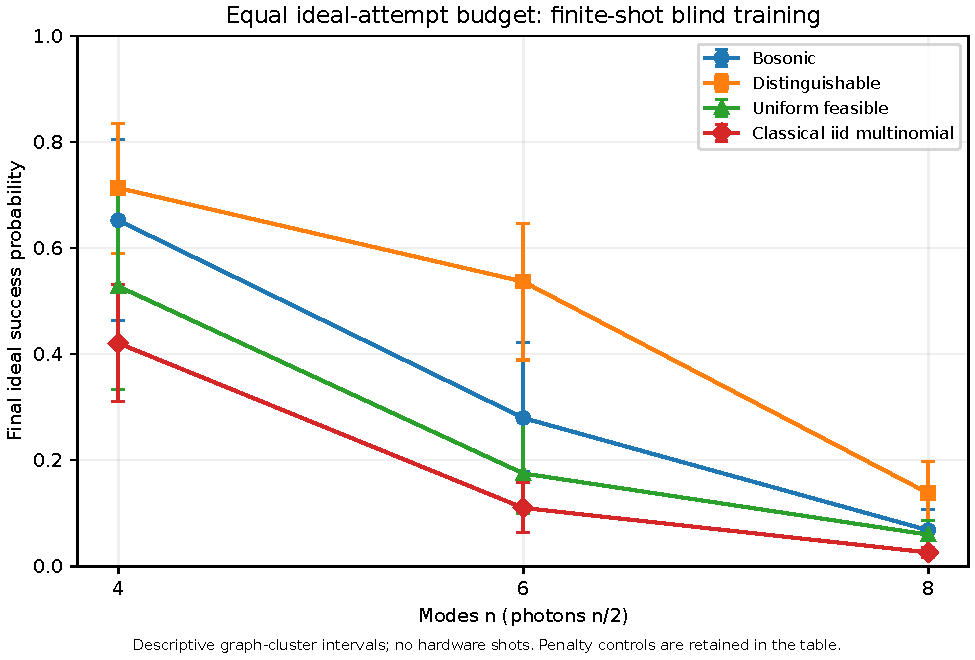
\includegraphics[width=.94\linewidth]{figures/fig_e05b.pdf}
 \caption{Final success of bosonic and distinguishable E05b procedures, with the complete nominal-grid means shown as points. Descriptive intervals resample whole graph clusters, retaining optimizer repeats and nominal-slot multiplicities; they are not a population confidence claim for random graph ensembles. Per-graph and per-seed values, penalty settings and aggregation rules are supplied with the data.}\label{fig:e05b}
\end{figure}

The bosonic final means are lower than the distinguishable means at all three sizes. These observations reject the claimed benefit for this implementation on this grid and budget; they do not prove that every optical optimizer is inferior. Every archived run already encounters an optimal solution during training, so the final circuit probability alone fails to describe problem-solving utility. Count traces locate the first \emph{winning batch}, but do not preserve shot order inside a batch. Exact first-hit shot counts cannot be recovered and are not imputed. Thus a claim of shorter time to first optimum is not supported by these data. A future search trial must save ordered queries and charge preprocessing, restarts, training, final samples and decoding.

The uniform balanced sampler is a relevant feasibility baseline; Bernoulli penalties are a different, weaker control and their three strengths are reported separately. The P21 classical search archive supplies balanced random search, exchange/local improvement and graph-aware controls at a separate cut-query budget. Spectral preprocessing and graph relabeling tests show why a successful optically encoded sample can inherit classically supplied graph structure. These campaigns strengthen the no-benefit assessment, but their differing budgets do not form a matched wall-clock speedup experiment. The new evidence inventory gives their exact provenance and resource units.

ObliQ is an actual hybrid photonic QUBO algorithm~\cite{ranjan2025}, not a synonym for an independent Bernoulli sampler. The authenticated static optical kernel was checked against its archive, Fock calculations and Perceval; literal and physically corrected angle conventions are kept separate. Complete original training, source selection and prefix decoding have not been reproduced, so no end-to-end superiority over authentic ObliQ is claimed.

\subsection{Finite theory checks and retained counterexamples}
The accepted supervised P33 primary/replication data cover all $300$ registered grid circuits, with full-law computations restricted to at most twelve modes; an additional $72$ entries evaluate certificate quantities only. Larger-frame entries evaluate certificate quantities only. Independent complete-law and Perceval controls support implementation consistency within stated tolerances, without proving the theorem. \Cref{fig:density} is generated from those accepted files; unattributed root-level P33 copies are excluded.
\begin{figure}[tb]
 \centering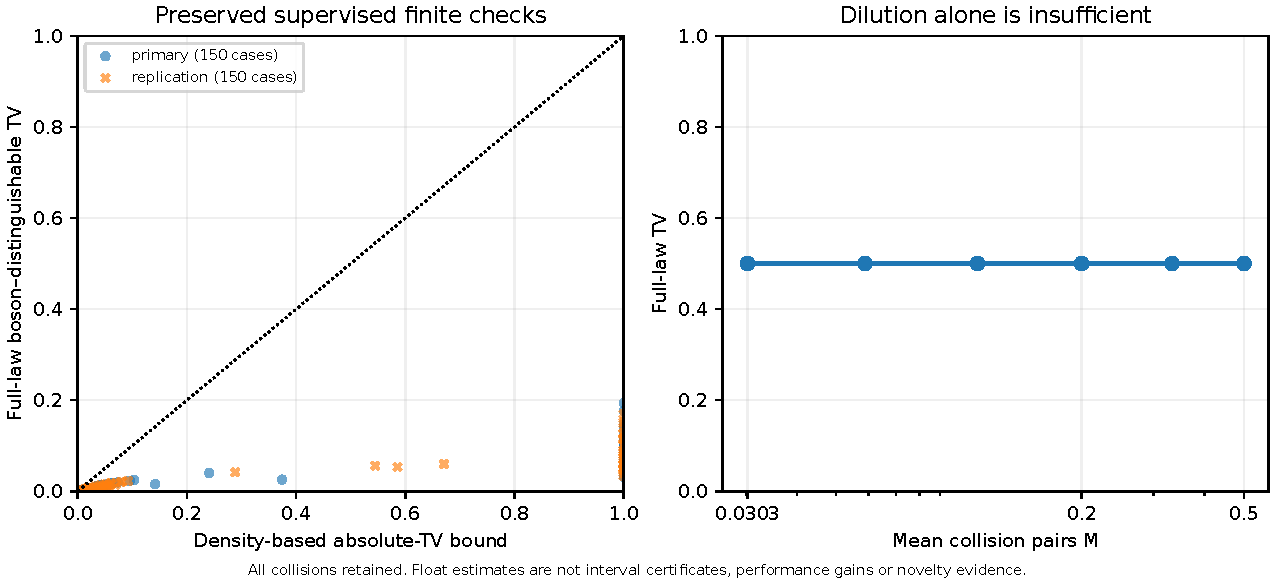
\includegraphics[width=\linewidth]{figures/fig_density.pdf}
 \caption{Left: 300 complete-law grid checks against the coarse density envelope $\Phi(M/c)$ from the accepted supervised primary/replication archive. Right: dilute spectator controls with decreasing collision-pair moment and constant TV. Separate sharp-family and certificate-only large-frame entries are retained in the data; the latter are not full-law comparisons. The sharp family and spectator obstruction test different hypotheses of \cref{thm:density}.}\label{fig:density}
\end{figure}

The P35 low-rank threshold expectation calculation is an exact classical mean-objective control, consistent with known product-state counting methods~\cite{ivanov2020}; it is not a sampler or a new optimization algorithm. Its earlier resource-guard defect and independent post-fix receipt are preserved. A stronger proposed pinched-state curved envelope was refuted in P39 by an exact physical three-photon/nine-mode construction at leakage $18/25$. Its measured output total variation remains below that curve: the refutation concerns the larger auxiliary state metric. The general measured bound $\TV\le\delta$ remains open. Failed searches and nonconverged solvers are retained as such, not promoted into proofs.

\section{Noise model and a prospective hardware pilot}\label{sec:pilot}
\subsection{Physical noise scenarios}
The recovered simulator retains all loss sectors, including vacuum, under uniform independent survival. It can equivalently average over independently surviving input subsets before applying the passive unitary. Uniform loss gives \cref{eq:all_detected} for a direct valid event; specified output-mode losses can also be applied after the unitary and cannot generally be commuted through it. Internal component losses, dark counts and detector saturation need additional models. A direct-sum matrix $\sqrt\eta U\oplus\sqrt{1-\eta}I$ is not a unitary dilation and is not used.

Partial distinguishability is specified by normalized pure internal states $|\phi_a\rangle$ with Hermitian positive-semidefinite Gram matrix $S_{ab}=\langle\phi_a|\phi_b\rangle$, $S_{aa}=1$. For distinct occupied inputs the double-permutation expression is
\begin{equation}
 p_S(t)=\frac1{t!}\sum_{\sigma,\tau\in S_k}
 \prod_{j=1}^k V_{y_j,\sigma(j)}\overline{V_{y_j,\tau(j)}}
 S_{\tau(j),\sigma(j)}.\label{eq:partial}
\end{equation}
This convention yields $p_b$ for $S_{ab}=1$ and $p_d$ for $S=I_k$, and retains multiphoton phases~\cite{tichy2015}. A single global mixture $\xi p_b+(1-\xi)p_d$ is not its general $k\ge3$ form. For a balanced two-port coupler, the coincidence probability is $(1-|S_{12}|^2)/2$. Pair overlaps alone do not determine every higher-order internal phase. The implemented small-system model assumes product pure internal states and distinct inputs; it is not a calibration of a particular device. Tests include independent internal-mode creation calculations and local Perceval controls. No broad noise-optimization campaign is asserted.

\subsection{A calibration prediction tied to the certificate}
The sharp family in \cref{eq:sharp} provides a second-stage target beyond identity and HOM. Let $M_0=2\cos^2\theta\sin^2\theta$, let $x=|S_{12}|^2$ and let $\eta$ be uniform transmission. Its complete detected law $p_{x,\eta}$ obeys
\begin{equation}
 \TV(p_{x,\eta},p_{0,\eta})=\eta^2 xM_0,\qquad
 P_{\rm collision}(x,\eta)=\succp^{\rm path}(x,\eta)
 =\frac{\eta^2(1+x)M_0}{2}.\label{eq:calibration}
\end{equation}
Here the natural path has vertices $0$--$1$--$2$--$3$, and its two optimal strings put both photons in one of the two mode groups. The two-photon law interpolates linearly in $x$, while its zero- and one-photon loss sectors are identical for all $x$. These facts and \cref{eq:sharp} prove \cref{eq:calibration}; this two-photon interpolation is not a general multiphoton noise ansatz.

The registered P40 local check fixes five rational rotation parameters:
\begin{gather*}
 r\in\{0,1/20,1/10,1/5,1/3\},\\
 \cos\theta=(1-r^2)/(1+r^2),\qquad \sin\theta=2r/(1+r^2).
\end{gather*}
It tests transmissions $\eta\in\{1,0.9,0.5\}$ and overlaps $x\in\{0,1/2,1\}$. All \CalibrationCellCount{} cells are retained without fitting, sampling or optimization. Its exported circuit first mixes the occupied inputs by $\mathrm{BS.Rx}(4\arctan r)$, permutes modes $(0,2,1,3)$, and splits each mode group by $\mathrm{BS.Rx}(\pi/2)$. Output phases do not affect the displayed laws. The script, complete loss-sector laws, unitary/circuit exports, advance contract and execution receipt are supplied separately.

This family can display a same-circuit twofold success ratio. A uniformly selected feasible Fock string that is then optically prepared and transmitted has success $\eta^2/3$, while a standalone classical uniform balanced sampler succeeds with probability $1/3$ per classical draw and incurs no optical loss. These resource units differ. An optically prepared known-optimum identity control has success $\eta^2$. The latter is a state-preparation diagnostic, not an unknown-optimum search. A measurable interference effect therefore does not establish optimization benefit. Under loss, the fixed-$k$ theorem must not be applied directly to uncorrected lower-sector moments. The proposed device test needs independently supported uniform-loss/internal-overlap assumptions and actual detector/attempt calibration.

\subsection{A falsifiable four-mode measurement}
The proposed initial device question is modest: can a calibrated processor reproduce a predicted two-photon occupation law and the resulting change in valid-cut probability under controlled overlap? Identity, a balanced Hong--Ou--Mandel circuit, and a fixed pair-mixing circuit form a four-mode/two-photon pilot. Paths, $K_4$ and $K_{2,2}$ separate graph decoding from optical interference. The $K_4$ control is deliberately uninformative about quality enrichment because every balanced cut is optimal.

The offline pipeline performs graph validation, generates full complex unitaries and parameters, constructs serializable Perceval circuits, checks local compilation and reference distributions, prepares a non-submitting job bundle and analyzes supplied counts. Circuit equivalence is checked up to global phase with mode ordering retained. It does not imply acceptance by a remote backend's gate set. The manifest seals circuit, reference, graph, convention and software hashes. Synthetic demonstration counts are explicitly labeled \texttt{local\_synthetic}; they are never called QPU data.

To estimate success per injected attempt, retain a trustworthy number of attempts together with all recorded occupancies and filter metadata. PNR data can separate bunching from loss directly under a calibrated model. Threshold data cannot generally reconstruct an arbitrary number distribution; the observable and event definition must match the detector. If only postselected counts are supplied, the analysis reports conditional probabilities and leaves attempt-normalized success unidentified. Per-event Wilson intervals are marginal binomial intervals, not a simultaneous goodness-of-fit test. Finite-shot density certification additionally needs controlled uncertainty in $M$, $c$ and model assumptions; the offline pilot does not solve that inference problem.

The handoff includes commands, fixed inputs, local references, expected schemas and explicit questions for the hardware operator. Public documentation and a local Perceval version do not establish this account's backend availability, mode count, native Clements mesh, detector resolution, shot API, calibration or credit cost. These remain verification items. No remote processor was instantiated, no device job was submitted, and no hardware measurements enter this paper.

\section{Discussion and conclusion}\label{sec:discussion}
The main certificate explains a limited operational implication of collisions: with a controlled minimum positive row intensity and sufficiently small expected pair moment, independent particles approximate the full bosonic law with a dimension-independent absolute error. The balanced sharp family fixes its leading coefficient at $c=1/2$. The spectator construction shows why low collision probability at balanced average density does not imply that approximation. This combination prevents an experiment from using a single collision statistic as a general witness of computational hardness or usefulness.

The result is a sufficient approximation by a specific efficiently sampled comparator. Other classical algorithms can reproduce laws for which the certificate is vacuous. Absolute event error does not control relative rare-event gains, and same-circuit comparison does not substitute for retraining the classical control. Haar source selection similarly changes feasibility and resource consumption without enriching graph quality. These distinctions account for why a mathematically positive certificate and a negative optimization benchmark are consistent.

The empirical result concerns fixed small graphs and budgets, with duplicate graph seeds, small graph counts and incomplete within-batch ordering. It supports no statement about asymptotic advantage or all photonic ansatz families. Exact reference simulation has substantial classical cost and is not a free experimental oracle. The archived spectral and label controls expose additional routes by which supplied classical information can dominate the apparent optical mechanism. The present implementation has not demonstrated the originally sought optimization benefit.

Several obligations remain before a strong research submission. Originality and significance of the complete density composition require independent literature assessment beyond the bounded source comparisons. Statistical certification from imperfect hardware needs a nonasymptotic uncertainty treatment and justified density support. An end-to-end optimization claim needs an optimum-blind mechanism, ordered total-cost traces, representative held-out graph labels and stronger classical controls under explicitly matched resource criteria. Authentic ObliQ training and decoding remain a separate reproduction task. Author metadata and the target venue require confirmation before circulation.

The current output is a reproducible theory-and-methodology manuscript, not a certified quantum-advantage or completed hardware paper. The offline pilot makes the next physical test concrete: validate the small occupation law and its denominators before using hardware to evaluate a new search hypothesis.

\bibliographystyle{plain}
\bibliography{references}
\appendix
\section{Full-output permanent and cycle bounds}\label{app:gram}
For a fixed ordered output list $y$ put $a_\sigma(y)=\prod_jV_{y_j,\sigma(j)}$ and $F(y)=\sum_{\sigma\ne\tau}|a_\sigma(y)a_\tau(y)|$. Subtract the diagonal terms of \cref{eq:laws}, then apply the triangle inequality. There are $k!/t!$ ordered lists with occupation $t$, and $F$ is invariant under their permutations. Therefore
\begin{align}
 2\TV(p_b,p_d)&\le\sum_t\frac{F(y(t))}{t!}
 =\frac1{k!}\sum_{y\in[m]^k}\sum_{\sigma\ne\tau}|a_\sigma(y)a_\tau(y)|\nonumber\\
 &=\frac1{k!}\sum_{\sigma\ne\tau}\prod_j B_{\sigma(j),\tau(j)}
 =\sum_{\pi\ne\mathrm{id}}\prod_a B_{a,\pi(a)}=\per B-1.
\end{align}
Each relative permutation occurs $k!$ times; repeated output rows are included. This proves the first bound with the halved-TV convention.

For $A=B-I_k$, the coefficient of $z^r$ in $\per(I_k+zA)$ counts weighted permutations moving $r$ indices. Such a permutation is a disjoint collection of directed simple cycles of length at least two. Allowing cycles to overlap or repeat only increases coefficients, since all entries are nonnegative. If $C_\ell$ is the total weight of simple cycles of length $\ell$, counted up to cyclic rotation,
\begin{equation}
 \per(I_k+zA)\preceq\exp\left(\sum_{\ell=2}^k C_\ell z^\ell\right)
 \preceq\exp\left(\sum_{\ell=2}^\infty\frac{\operatorname{tr}(A^\ell)}\ell z^\ell\right).
\end{equation}
The relation is coefficientwise: every disjoint collection appears with coefficient one in the exponential, and all extra closed walks have nonnegative weights. Real symmetry gives
\begin{equation}
 0\le\operatorname{tr}(A^\ell)\le\sum_j|\lambda_j(A)|^\ell
 \le\left(\sum_j\lambda_j(A)^2\right)^{\ell/2}=\sigma^\ell\quad(\ell\ge2).
\end{equation}
The first inequality also holds for odd powers by the closed-walk expansion. Since
\begin{equation}
 \exp\left(\sum_{\ell\ge2}\frac{x^\ell}{\ell}\right)
 =\frac{e^{-x}}{1-x}=\sum_{r\ge0}\frac{!r}{r!}x^r,
\end{equation}
comparison through degree $k$ gives the finite polynomial bound for every $\sigma\ge0$. Summing the infinite envelope requires $\sigma<1$. These steps prove \cref{lem:gram} without an external theorem dependency. Computing $B$ costs $O(mk^2)$ arithmetic operations, and the finite bound another $O(k)$ once derangements are available. The comparator draws $k$ independent categorical outcomes and forgets labels after $O(mk)$ table preparation. This computational sufficiency does not extend the theorem to finite experimental uncertainty.

\section{Source crossings and the boundary expansion}\label{app:source}
\begin{lemma}[Single sign change under a binomial mixture]\label{lem:crossing}
Let $c_0,\ldots,c_n$ have positive entries followed by negative entries, allowing zeros, with both signs present. If the last nonzero coefficient is negative, $\E c_R$, $R\sim\mathrm{Bin}(n,\eta)$, has exactly one zero in $0<\eta<1$, crossing from positive to negative.
\end{lemma}
\begin{proof}
Set $t=\eta/(1-\eta)$. Remove the positive factor $(1-\eta)^n$ and let $a$ be the first negative coefficient index in $Q(t)=\sum_r\binom nr c_rt^r$. Then $Q(t)/t^a$ is strictly decreasing: positive terms have negative powers and negative terms have nonnegative powers. Its limit at zero is positive infinity and its limit at infinity is strictly negative or negative infinity. This proves existence, uniqueness and sign orientation.

For a fixed sign-pattern sequence, increasing $n$ strictly decreases the root when newly included coefficients are negative. For $0\le r\le n$, the ratio of binomial masses for $n+1$ and $n$ is $(1-\eta)(n+1)/(n+1-r)$, strictly increasing in $r$. At a zero of the old expectation, subtract its value at the sign boundary times that zero. Products of the remaining ratio differences with $c_r$ are nonpositive and at least one is strictly negative. The new $r=n+1$ contribution is negative. Hence the new expectation is negative at the old root; its own unique root is smaller.
\end{proof}

For \cref{thm:source}, $d(\ell)=h(\ell+1)-h(\ell)$ is zero below $k-1$, positive for $k-1\le\ell\le m-3$, zero at $m-2$, and negative at $m-1$. This follows by subtracting one from the exact ratio:
\begin{equation}
 \frac{h(\ell+1)}{h(\ell)}-1=\frac{k(m-2-\ell)}{(\ell-k+1)(m+\ell)}\quad(\ell\ge k).
\end{equation}
Coupling the extra Bernoulli survival shows $S_{N+1}-S_N=\eta\E d(L)$, $L\sim\mathrm{Bin}(N,\eta)$. For $N\le m-2$, every term is nonnegative and some positive term has nonzero mass. For $N=m-1$, \cref{lem:crossing} supplies the unique $a_m$. At $\eta=1$, the lossless peak $h(m-2)=h(m-1)$ restores the stated endpoint tie.

Set $g(0)=0$, $g(\ell)=h(\ell)/\ell$ for $\ell\ge1$. Binomial size bias gives
\begin{equation}
 b_N=\eta\E g(R+1),\qquad b_{N+1}-b_N=\eta^2\E[g(R+2)-g(R+1)],\quad R\sim\mathrm{Bin}(N-1,\eta).
\end{equation}
For $\ell\ge k$, subtracting the denominator from the numerator of $g(\ell+1)/g(\ell)$ gives $[m(m-2)-(m+2)\ell]/2$, whose zero $m-4+8/(m+2)$ lies strictly between $m-4$ and $m-3$ for $m\ge8$. Thus $\Delta g(\ell)$ is zero below $k-1$, positive through $m-4$ and negative from $m-3$ through $m-1$. It follows that $b_N$ strictly increases through $N=m-3$. Applying the lemma to $c_r=\Delta g(r+1)$ proves each of the three remaining unique roots; its root-order argument gives $\tau_{m-1}<\tau_{m-2}<\tau_{m-3}$. These ordered adjacent signs make the candidate sequence strictly increase and then decrease. Nonadjacent candidates cannot create a missed global maximum. At $\eta=1$, $g$ has its unique integer maximum at $m-3$.

For the boundary scaling let $N=m-s$, $\eta=1-\lambda/m$, with $s,\lambda$ fixed and $m$ even tending to infinity. The loss count $T$ is $\mathrm{Bin}(m-s,\lambda/m)$ for the $h$ identity, or $\mathrm{Bin}(m-s-1,\lambda/m)$ after size bias for $g$. Its fixed moments are uniformly bounded, $\E T=\lambda+O(m^{-1})$, and each fixed positive exponential moment is bounded uniformly in $m$. On $\ell=m-s-T\ge3m/4$, the exact ratios yield
\begin{align}
 \Delta h(\ell)/h(\ell)&=(s+T-2)/(2m)+O((1+s+T)^2/m^2),\\
 \Delta g(\ell)/g(\ell)&=(s+T-4)/(2m)+O((1+s+T)^2/m^2).
\end{align}
Summing adjacent relative differences from the lossless peaks also gives $h(\ell)/h(m-1)=1+O((1+s+T)^2/m)$ and $g(\ell)/g(m-3)=1+O((1+s+T)^2/m)$. Peak-normalized values are bounded; the bounded number of indices above the $g$ peak causes no difficulty. The event $T>m/4-s$ has exponentially small probability by the exponential-moment bound. Functions and adjacent differences are bounded by constant multiples of their peaks, so this tail contributes $o(m^{-2})$ after normalization. Take expectations in the coupling identities and divide by their corresponding means to obtain \cref{eq:boundary}. Evaluating signs at $\lambda$ just above and below each proposed limit, then using unique crossings, gives the four scaled-root limits. This reasoning keeps $s,\lambda$ fixed and supplies no fixed-loss asymptotic.

\section{Reproduction, evidence and measurement conventions}\label{app:repro}
\paragraph{Single data source.}
The accepted recovery directory is \path{results/validated/} with dated subdirectory \path{recovery_2026-11-24/}. It contains \path{summary.json}, per-run \path{benchmark.csv}, campaign inventory and source hashes. The publication generator reads these and the pinned P33/P37 raw records, emits every numerical table, figure and macro used here, and writes \path{paper/publication_manifest.json}. Its check mode rejects stale sources or divergent generated tables. Constants in graph and analytic model tables are independently computed from their definitions. No hand-entered performance table is used.

\paragraph{Commands.}
With the pinned project extras installed, run the following from the repository root:
\begin{verbatim}
python scripts/reconcile_experiments.py --help
python scripts/build_publication.py
python scripts/build_publication.py --check
python -m pytest tests/ -q
tectonic --untrusted --keep-logs paper/main.tex
python -m photonic_balanced_partitioning.hardware --help
\end{verbatim}
The reconciliation help lists the exact destination rules; existing archived raw files are never targets. The source package pins numerical and Perceval dependencies. Tectonic is external build infrastructure. The execution report records the actually observed compiler, commands, test counts and source revision. No remote QPU is needed for this sequence.

\paragraph{Evidence boundaries.}
P33 and P37 have prior independent proof reviews of exact hashed statements; the revised paper is additionally reviewed across physics, optimization and reproducibility scopes. Finite tests, reviewers' agreement and compilation are not proofs of originality. Historical manuscripts and unsupported gain tables remain recoverable in Git, but are withdrawn from the current article. Some archive manifests have incomplete source snapshots; these limitations are explicit in the campaign inventory. No unavailable campaign is treated as newly replicated.

\paragraph{Observables.}
An emission attempt may fail before injection. A successfully injected $N$-photon trial may lose photons before detection. A detected occupation is a PNR vector, or a threshold click vector under a specified detector map. A collision-free occupation satisfies $t_i\le1$; a direct valid graph encoding additionally has $|t|=k$. An optimal event is valid and has cost $C^*$, used retrospectively on these exactly solvable small graphs. Conditional valid-event and attempt-normalized probabilities have distinct denominators. Raw hardware records, if later acquired, must be immutable; preprocessing, excluded events and denominator provenance belong in separate derived files.

\end{document}
